\section{Results}

\subsection{Truth Table}

Referring to the procedure, we can create the 7448 decoder's truth table as follows:

\begin{table}[h!]
    \centering
    \begin{displaymath}
        \begin{array}{|c c c c|c c c c c c c|}
        A & B & C & D    &   a & b & c & d & e & f & g\\
        \hline
        0 & 0 & 0 & 0    &   1 & 1 & 1 & 1 & 1 & 1 & 0\\
        0 & 0 & 0 & 1    &   0 & 1 & 1 & 0 & 0 & 0 & 0\\
        0 & 0 & 1 & 0    &   1 & 1 & 0 & 1 & 1 & 0 & 1\\
        0 & 0 & 1 & 1    &   1 & 1 & 1 & 1 & 0 & 0 & 1\\
        0 & 1 & 0 & 0    &   0 & 1 & 1 & 0 & 0 & 1 & 1\\
        0 & 1 & 0 & 1    &   1 & 0 & 1 & 1 & 0 & 1 & 1\\
        0 & 1 & 1 & 0    &   0 & 0 & 1 & 1 & 1 & 1 & 1\\
        0 & 1 & 1 & 1    &   1 & 1 & 1 & 0 & 0 & 0 & 0\\
        1 & 0 & 0 & 0    &   1 & 1 & 1 & 1 & 1 & 1 & 1\\
        1 & 0 & 0 & 1    &   1 & 1 & 1 & 0 & 0 & 1 & 1\\
        1 & 0 & 1 & 0    &   X & X & X & X & X & X & X\\
        1 & 0 & 1 & 1    &   X & X & X & X & X & X & X\\
        1 & 1 & 0 & 0    &   X & X & X & X & X & X & X\\
        1 & 1 & 0 & 1    &   X & X & X & X & X & X & X\\
        1 & 1 & 1 & 0    &   X & X & X & X & X & X & X\\
        1 & 1 & 1 & 1    &   X & X & X & X & X & X & X\\
        \end{array}
    \end{displaymath}
    \caption{Truth table of a 7448 decoder}
    \label{tab:my_label}
\end{table}

\subsection{Karnaugh Maps}

Referring to the procedure and the truth table, we can obtain minimized Boolean functions in sum-of-products form for each output (a-g) using Karnaugh Maps. The Karnaugh Maps will be on the left-hand side and the minimized Boolean functions will be on the right-hand side for the next subsections.

\subsubsection{Output: a}
\begin{minipage}{0.5\textwidth}
    \centering
    \begin{karnaugh-map}[4][4][1][$D$][$C$][$B$][$A$]
        \minterms{0, 2, 3, 5, 7, 8, 9}
        \maxterms{1, 4, 6}
        \terms{10, 11, 12, 13, 14, 15}{$X$}
        \implicantcorner
        \implicant{12}{10}
        \implicant{3}{11}
        \implicant{5}{15}
    \end{karnaugh-map}
\end{minipage}
\begin{minipage}{0.5\textwidth}
Simplified function in sum-of-products:
\[
a(A,B,C,D) = A + BD + \bar{B}\bar{D} + CD
\]
\end{minipage}

\subsubsection{Output: b}
\begin{minipage}{0.5\textwidth}
    \centering
    \begin{karnaugh-map}[4][4][1][$D$][$C$][$B$][$A$]
        \minterms{0, 1, 2, 3, 4, 7, 8, 9}
        \maxterms{5, 6}
        \terms{10, 11, 12, 13, 14, 15}{$X$}
        \implicantedge{0}{2}{8}{10}
        \implicant{3}{11}
        \implicant{0}{8}
    \end{karnaugh-map}
\end{minipage}
\begin{minipage}{0.5\textwidth}
Simplified function in sum-of-products:
\[
b(B,C,D) = \bar{B} + CD + \bar{C}\bar{D}
\]
\end{minipage}

\subsubsection{Output: c}
\begin{minipage}{0.5\textwidth}
    \centering
    \begin{karnaugh-map}[4][4][1][$D$][$C$][$B$][$A$]
        \minterms{0, 1, 3, 4, 5, 6, 7, 8, 9}
        \maxterms{2}
        \terms{10, 11, 12, 13, 14, 15}{$X$}
        \implicant{0}{9}
        \implicant{1}{11}
        \implicant{4}{14}
    \end{karnaugh-map}
\end{minipage}
\begin{minipage}{0.5\textwidth}
Simplified function in sum-of-products:
\[
c(B,C,D) = B + \bar{C} + D
\]
\end{minipage}

\subsubsection{Output: d}
\begin{minipage}{0.5\textwidth}
    \centering
    \begin{karnaugh-map}[4][4][1][$D$][$C$][$B$][$A$]
        \minterms{0, 2, 3, 5, 6, 8}
        \maxterms{1, 4, 7, 9}
        \terms{10, 11, 12, 13, 14, 15}{$X$}
        \implicantcorner
        \implicant{2}{10}
        \implicantedge{3}{2}{11}{10}
        \implicant{5}{13}
    \end{karnaugh-map}
\end{minipage}
\begin{minipage}{0.5\textwidth}
Simplified function in sum-of-products:
\[
d(B,C,D) = \bar{B}\bar{D} + \bar{B}C + C\bar{D} + B\bar{C}D
\]
\end{minipage}

\subsubsection{Output: e}
\begin{minipage}{0.5\textwidth}
    \centering
    \begin{karnaugh-map}[4][4][1][$D$][$C$][$B$][$A$]
        \minterms{0, 2, 6, 8}
        \maxterms{1, 3, 4, 5, 7, 9}
        \terms{10, 11, 12, 13, 14, 15}{$X$}
        \implicantcorner
        \implicant{2}{10}
    \end{karnaugh-map}
\end{minipage}
\begin{minipage}{0.5\textwidth}
Simplified function in sum-of-products:
\[
e(B,C,D) = \bar{B}\bar{D} + C\bar{D}
\]
\end{minipage}

\subsubsection{Output: f}
\begin{minipage}{0.5\textwidth}
    \centering
    \begin{karnaugh-map}[4][4][1][$D$][$C$][$B$][$A$]
        \minterms{0, 4, 5, 6, 8, 9}
        \maxterms{1, 2, 3, 7}
        \terms{10, 11, 12, 13, 14, 15}{$X$}
        \implicant{0}{8}
        \implicant{12}{10}
        \implicant{4}{13}
        \implicantedge{4}{12}{6}{14}
    \end{karnaugh-map}
\end{minipage}
\begin{minipage}{0.5\textwidth}
Simplified function in sum-of-products:
\[
f(A,B,C,D) = A + B\bar{C} + B\bar{D} + \bar{C}\bar{D}
\]
\end{minipage}

\subsubsection{Output: g}
\begin{minipage}{0.5\textwidth}
    \centering
    \begin{karnaugh-map}[4][4][1][$D$][$C$][$B$][$A$]
        \minterms{2, 3, 4, 5, 6, 8, 9}
        \maxterms{0, 1, 7}
        \terms{10, 11, 12, 13, 14, 15}{$X$}
        \implicant{12}{10}
        \implicant{4}{13}
        \implicant{2}{10}
        \implicantedge{3}{2}{11}{10}
    \end{karnaugh-map}
\end{minipage}
\begin{minipage}{0.5\textwidth}
Simplified function in sum-of-products:
\[
g(A,B,C,D) = A + B\bar{C} + \bar{B}C  + C\bar{D}
\]
\end{minipage}

\subsection{Circuit Implementation}

Referring to the simplified functions, we can implement the 7448 decoder as:

\begin{figure}[h!]
    \centering
    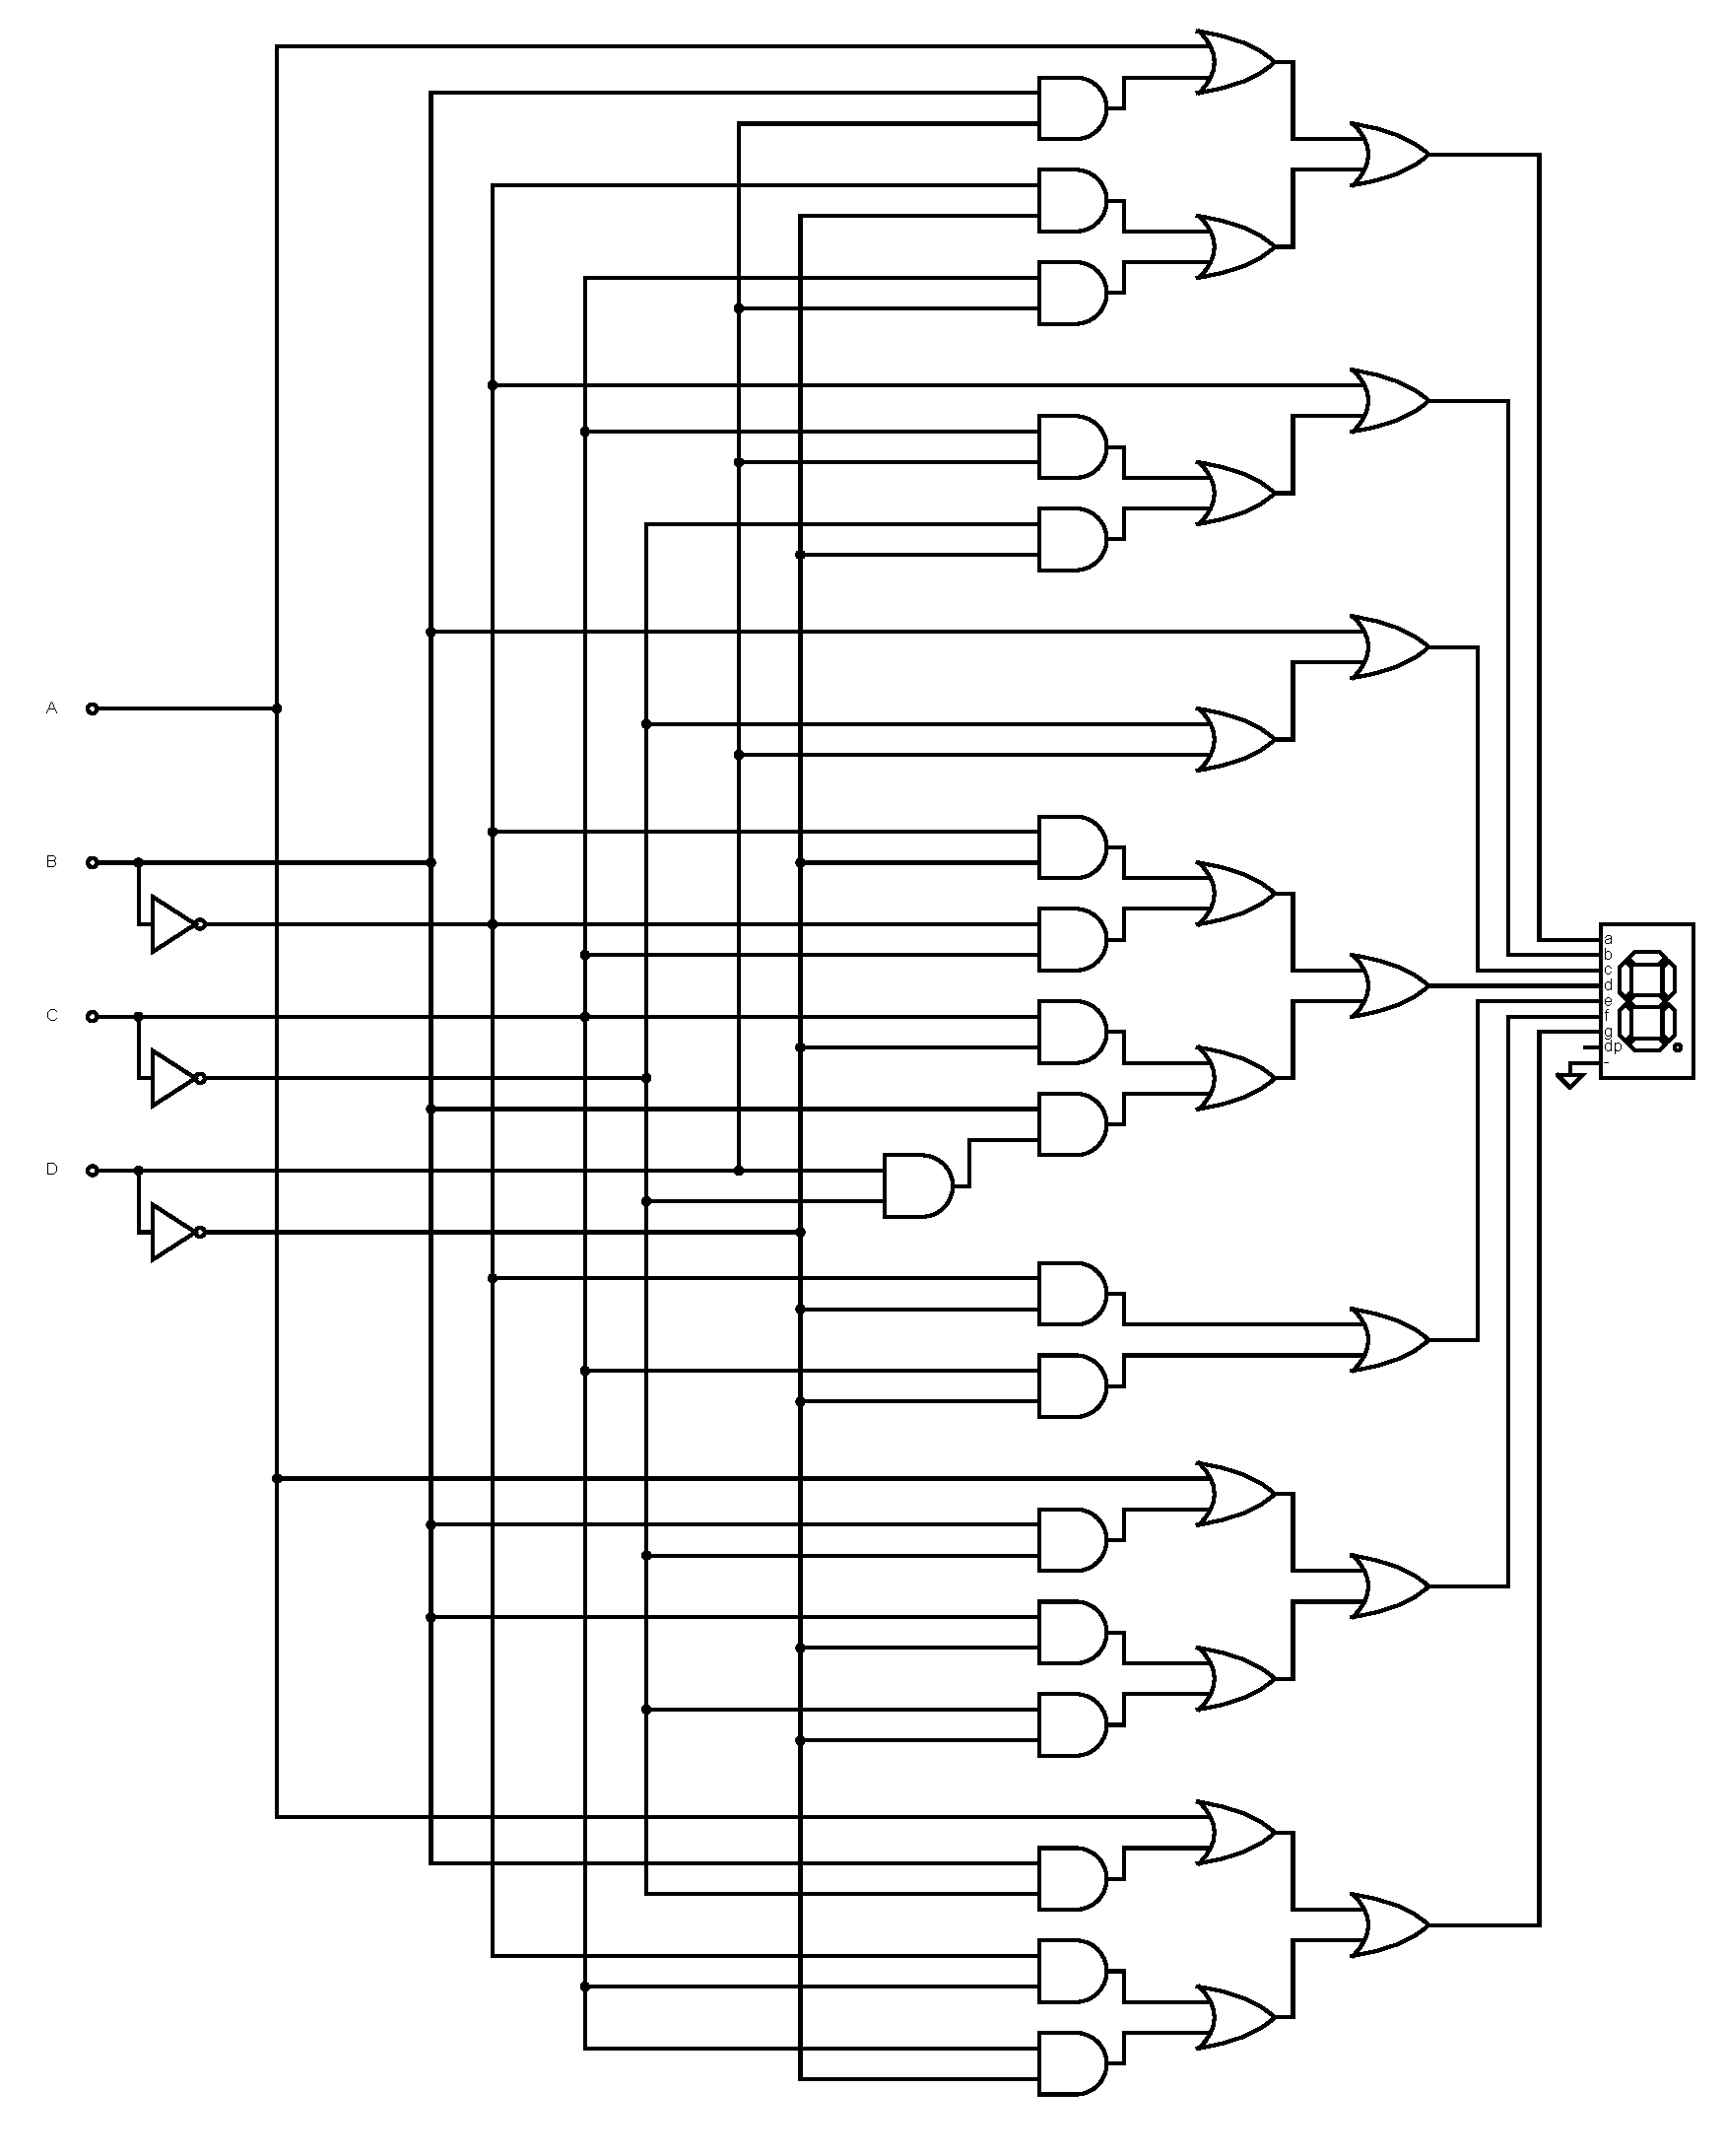
\includegraphics[width=0.8\textwidth]{images/7-segment-decoder.pdf}
    \caption{Circuit diagram of a 7448 decoder}
    \label{fig:your-label}
\end{figure}
